% VLDB template version of 2020-08-03 enhances the ACM template, version 1.7.0:
% https://www.acm.org/publications/proceedings-template
% The ACM Latex guide provides further information about the ACM template

\documentclass[sigconf, nonacm]{acmart}
\usepackage{mathtools}
\usepackage{xcolor}
\usepackage{graphicx}
\usepackage{multicol}
\usepackage{multirow}
\usepackage{amsfonts}
\usepackage{caption}
\usepackage{subfig}
\usepackage{changepage}
\usepackage{amsthm}

%% The following content must be adapted for the final version
% paper-specific
\newcommand\vldbdoi{XX.XX/XXX.XX}
\newcommand\vldbpages{XXX-XXX}
% issue-specific
\newcommand\vldbvolume{14}
\newcommand\vldbissue{1}
\newcommand\vldbyear{2020}
% should be fine as it is
\newcommand\vldbauthors{\authors}
\newcommand\vldbtitle{\shorttitle} 
% leave empty if no availability url should be set
\newcommand\vldbavailabilityurl{URL_TO_YOUR_ARTIFACTS}
% whether page numbers should be shown or not, use 'plain' for review versions, 'empty' for camera ready
\newcommand\vldbpagestyle{plain} 

% Andrew Macros
\newcommand\ourmethod{Uniform UMAP }
\newcommand{\centered}[1]{\begin{tabular}{l} #1 \end{tabular}}

\begin{document}
\title{A Thorough Analysis of and Improvement on UMAP and tSNE}

%%
%% The "author" command and its associated commands are used to define the authors and their affiliations.
\author{Andrew}
\author{Jakob}
\author{Katrine}
\affiliation{%
  \institution{Aarhus University}
  \streetaddress{Somewhere 5}
  \city{Aarhus}
  \state{}
  \postcode{8000}
  \country{}
}
\email{draganovandrew@cs.au.dk}
%%
%% The abstract is a short summary of the work to be presented in the
%% article.
\begin{abstract}
TSNE and UMAP have become two of the most popular dimensionality reduction algorithms due to their quick runtimes and intuitive low-dimensional embeddings.
Despite their ubiquity and similarities, however, there has not been a comprehensive attempt to fuse the two approaches into a single method. In this work, we
describe a general framework for comparing dimensionality reduction algorithms and analyze the differences between TSNE and UMAP in terms of this framework.
Under this framework, we identify which changes are necessary and sufficient to switch between the two approaches and disprove several claims regarding the
reason for each algorithms' efficacy, thus clarifying misconceptions regarding each algorithm.

Inspired by this, we create a new dimensionality reduction algorithm, \ourmethod, that combines the best characteristics of tSNE
and UMAP and is able to reproduce the results of either method with only a few hyperparameter changes. \ourmethod, when executed in a single thread, performs the optimization an order of magnitude faster than
multi-threaded UMAP and several orders of magnitude faster than multi-threaded tSNE on even modestly sized datasets. By virtue of its scalable characteristics,
we are able to effectively parallelize \ourmethod to obtain additional speed improvements. We also devise a new GPU
solution that performs our method's optimization significantly faster than existing GPU implementations of either UMAP or tSNE.

We lastly provide theoretical insights for future dimensionality reduction improvements. Our code is fully plug-and-play with the standard UMAP and tSNE
libraries and available to the public at \_\_\_\_.
\end{abstract}

\maketitle

%%% do not modify the following VLDB block %%
%%% VLDB block start %%%
\pagestyle{\vldbpagestyle}
\begingroup\small\noindent\raggedright\textbf{PVLDB Reference Format:}\\
\vldbauthors. \vldbtitle. PVLDB, \vldbvolume(\vldbissue): \vldbpages, \vldbyear.\\
\href{https://doi.org/\vldbdoi}{doi:\vldbdoi}
\endgroup
\begingroup
\renewcommand\thefootnote{}\footnote{\noindent
This work is licensed under the Creative Commons BY-NC-ND 4.0 International License. Visit \url{https://creativecommons.org/licenses/by-nc-nd/4.0/} to view a copy of this license. For any use beyond those covered by this license, obtain permission by emailing \href{mailto:info@vldb.org}{info@vldb.org}. Copyright is held by the owner/author(s). Publication rights licensed to the VLDB Endowment. \\
\raggedright Proceedings of the VLDB Endowment, Vol. \vldbvolume, No. \vldbissue\ %
ISSN 2150-8097. \\
\href{https://doi.org/\vldbdoi}{doi:\vldbdoi} \\
}\addtocounter{footnote}{-1}\endgroup
%%% VLDB block end %%%

%%% do not modify the following VLDB block %%
%%% VLDB block start %%%
\ifdefempty{\vldbavailabilityurl}{}{
\vspace{.3cm}
\begingroup\small\noindent\raggedright\textbf{PVLDB Artifact Availability:}\\
The source code, data, and/or other artifacts have been made available at \url{\vldbavailabilityurl}.
\endgroup
}
%%% VLDB block end %%%

\section{Introduction}
Dimensionality reduction (DR) algorithms are invaluable for qualitatively inspecting high-dimensional data and are used across computational and natural-science
disciplines for data visualization, denoising, graph embeddings, and many other tasks \textcolor{red}{REFERENCES}. Intuitively, DR algorithms accept a high-dimensional dataset as
input and find a faithful embedding in a lower-dimensional space. The term \textit{faithful} traditionally implies keeping similar points similar and dissimilar
points dissimilar, where similarity is measured by distance metrics or kernels in the corresponding spaces. This naturally implies a $O(n^2)$ runtime for many
nonlinear approaches, as we must compare the high- and low-dimensional pairwise distance matrices before we can be certain of the embedding quality.

Recent gradient-based methods have managed to improve on this by performing optimization only on relevant entries of the pairwise distance matrices.
Among these, TSNE and UMAP are by far the most popular due to their speed and intuitive results, each getting cited more than 1000 times per year on average.
They specifically overcome the $O(n^2)$ bound by constructing a setting in which distant points do not exert strong forces on one another, allowing the optimization to focus on nearest neighbors in the high dimensional space and sampling methods in the low-dimensional space.

Formally, TSNE \cite{van2008visualizing} and UMAP \cite{mcinnes2018umap} both receive an input dataset $X \in \mathbb{R}^{N \times D}$ of
$N$ points in $D$ dimensional space and
attempt to find a faithful embedding into a lower dimensional space $Y \in \mathbb{R}^{N \times d}$, where $d << D$. 
 In this paper, we refer to the pairwise squared distance matrices in high- and low-dimensional spaces as $E^X$ and $E^Y$, respectively. Both algorithms then define high-
 and low-dimensional non-linear functions $p: X \times X \rightarrow [0, 1]$ and $q: Y \times Y \rightarrow [0, 1]$, giving us pairwise similarity matrices $P$
 and $Q$. For both algorithms, $p$ is an inverse exponential function while $q$ is an inverse polynomial function --- these are chosen specifically to handle
 differences between high- and low-dimensional distance distributions. Subject to normalization, the similarity matrices carry a probabilistic interpretation,
 allowing TSNE and UMAP to model the dimensionality reduction problem as minimizing the KL divergence $KL(P || Q)$ and optimizing by gradient descent. In
 practice, this amounts to iteratively applying attractive and repulsive forces with respect to the differing values between $P$ and $Q$.

Despite their ubiquity and similarity, however, there has not yet been a comprehensive attempt to unify the two methods for several reasons.
First, the algorithms are presented in radically different ways. While TSNE is described from a computational perspective, UMAP is instead introduced with
a littany of category theory and topology proofs. Second, many of the differing design choices do not have accompanying theoretical descriptions. For example,
TSNE calculates the repulsion acting on point $y_i$ to every other point $y_j$ while UMAP calculates repulsions to only a constant number of points. This means
TSNE's is then more in line with the gradient derivation while UMAP's is computationally more efficient. It is unclear, however, whether one could instead
perform TSNE with UMAP's repulsions or vice-versa and the necessary algorithmic changes are non-trivial to implement. These kinds of questions arise for many
discrepancies between the algorithms such as their initialization, the normalization of $P$ and $Q$, the symmetrization, etc.

\begin{figure*}[h]
    \begin{tabular}{cc}
        \includegraphics[width=.24\linewidth]{outputs/mnist/tsne/default/embedding.png}\par
        \includegraphics[width=.24\linewidth]{outputs/mnist/uniform_umap/normalized/embedding.png}\par
        \includegraphics[width=.24\linewidth]{outputs/mnist/uniform_umap/default/embedding.png}\par
        \includegraphics[width=.24\linewidth]{outputs/mnist/umap/default/embedding.png}\\
        \includegraphics[width=.24\linewidth]{outputs/fashion_mnist/tsne/default/embedding.png}\par
        \includegraphics[width=.24\linewidth]{outputs/fashion_mnist/uniform_umap/normalized/embedding.png}\par
        \includegraphics[width=.24\linewidth]{outputs/fashion_mnist/uniform_umap/default/embedding.png}\par
        \includegraphics[width=.24\linewidth]{outputs/fashion_mnist/umap/default/embedding.png}
    \end{tabular}
\caption{Uniform UMAP is able to recreate both TSNE and UMAP embeddings by just changing two hyperparameters. Images above are on the MNIST (top row) and
Fashion MNIST (bottom row) datasets. From left to right: TSNE, \ourmethod with normalization, \ourmethod and UMAP}
\end{figure*}

Towards the goal of unifying TSNE and UMAP, we first identify every framework choice and implementation discrepancy between the two methods. This allows us to describe each algorithm as a set of on/off
switches across the space of these differences. We then implement tSNE and UMAP in a common library, giving us the ability to study the effect of these
''switches`` on each of the algorithms.
We provide evidence that the most relevant change is the choice of normalization on the pairwise similarity matrices $P$ and $Q$ along with the corresponding
necessary gradient descent modifications.
In fact, a majority of the differences between TSNE and UMAP turn out to be negligible in terms of both quantitative and qualitative effects across datasets.
This raises questions regarding several claims that have been made regarding the necessary computational components of the two methods.

Based on this analysis we propose \ourmethod, an embedding algorithm that recreates both tSNE and UMAP embeddings by changing just two input parameters.
We experimentally validate that \ourmethod can simulate both methods through quantitative metrics and qualitative
evaluations. Surprisingly, we also show that the choice of optimizing the KL divergence is not set in stone, finding that minimizing the Frobenius norm provides
embeddings of a similar quality despite significantly simpler gradient calculations. Due to these improvements, \ourmethod is particularly amenable to
parallelization, recreating UMAP's embeddings 5-times faster and TSNE's several orders of magnitude faster.
Lastly, our library includes the option for GPU code, giving us the fastest method for optimizing TSNE and UMAP embeddings in any algorithm/processor setting.
Our code is fully compatible with each algorithm's current popular implementation and is available at \_\_\_\_.

In summary, our contributions are as follows:
\begin{enumerate}
        \item We perform the first full analysis of every difference between the TSNE and UMAP algorithms, identifying which changes are necessary to
        convert one algorithm to the other.
        \item We propose \ourmethod, an optimization algorithm that effectively recreates either TSNE or UMAP embeddings as dictated by only two input
            parameters.
        \item We release a simple, plug-and-play implementation of our approach, providing significant speed improvements for TSNE and UMAP on both
        the CPU and GPU.
\end{enumerate}

\section{Related Work}

\ourmethod falls into a broad category of gradient based DR approaches, characterized by minimizing a non-convex objective using variants of gradient descent.
We have already presented TSNE and UMAP, which are the two most common, but there exist several variations on each of these algorithms. When discussing TSNE, we
refer to \cite{van2014accelerating}, which established the nearest neighbor and sampling speed improvements. Since this paper, a popular subsequent improvement
was presented in \cite{linderman2019fast}, wherein Fast Fourier Transforms were used to accelerate the comparisons between points. Another approach based on
TSNE is the LargeVis algorithm, proposed in \cite{tang2016visualizing}, which modifies the embedding functions to satisfy a graph-based Bernoulli probabilistic model of
the low-dimensional dataset. As the more recent algorithm, UMAP has not had as many variations yet. One promising direction, however, has been to extend the
second step of UMAP as a parametric optimization on neural network weights \cite{sainburg2020parametric}.

Many of these approaches utilize the same optimization structure where they iteratively attract and repel points. While most perform their attractions similarly
along nearest neighbors in the high-dimensional space, it is the repulsions that are the slowest operation and that each method approaches differently.
The original TSNE method samples repulsions by utilizing Barnes-Hut trees to sum the effects of distant points from one another.
The work by Linderman et. al instead calculates repulsive forces with respect to specifically chosen 'interpolation` points, cutting down on the $O(nlogn)$
requirement of the tree calculations at every gradient step. UMAP and LargeVis, on the other hand, simplify the repulsion sampling by only calculating the
gradient with respect to a constant number of points. These techniques are, on their face, incompatible with one another -- several modifications have to be made
to each algorithm before one can easily interchange one repulsive force calculation for another.

While modifying the algorithms is more challenging, there have been several papers that attempt to explain the difference between TSNE and UMAP by looking at
other algorithmic design choices. In both \cite{kobak2019umap} and \cite{kobak2021initialization},
the argument is made that the necessary and sufficient condition to switch between their embeddings is the difference in initialization between the two methods.
Namely, TSNE randomly initializes the low dimensional dataset whereas UMAP first calculates a Laplacian Eigenmap \cite{belkin2003laplacian} embedding before
beginning the optimization. We have been unable to reproduce these results across datasets and optimization criteria, a topic we discuss later in our results.

Lastly, we also mention the state-of-the-art implementations of both TSNE and UMAP on the GPU. The CPU implementations are found in the scikit-learn and
umap-learn python libraries for TSNE and UMAP, respectively. The fastest current implementations on the GPU, however, can be found in the RAPIDS AI
framework \cite{nolet2020bringing} \cite{rapidsframework}.




\section{Comparison of tSNE and UMAP} \label{comparison}
We begin by formally introducing the tSNE and UMAP DR algorithms. Let $X \in \mathbb{R}^{N \times D}$ be the high dimensional dataset of $N$ points and let $Y
\in \mathbb{R}^{N \times d}$ be a previously initialized set of $N$ points in lower-dimensional space such that $d << D$. 

We now respectively establish Gaussian and student-t kernels on the high- and low-dimensional distances to represent the similarities between points $x_i$,
$x_j$ and $y_i$, $y_j$. These kernels are defined as
\begin{align}
    % FIXME - the denominator here isn't quite right
    p^{tsne}_{j|i}(x_i, x_j) &= \dfrac{\text{exp}(-d(x_i, x_j)^2 / 2 \sigma_i^2)}{\sum_{k \neq l} \text{exp}(-d(x_k, x_l)^2 / 2 \sigma_k^2)} \\[0.5ex]
    q^{tsne}_{ij}(y_i, y_j) &= \dfrac{(1 + ||y_i - y_j||^2_2)^{-1}}{\sum_{k \neq l} (1 + ||y_k - y_l||^2_2)^{-1}} \\[1.5ex]
    p^{umap}_{j|i}(x_i, x_j) &= \text{exp} (-d(x_i, x_j)^2 + \rho_{i}) /\tau_i \\[0.3ex]
    q^{umap}_{ij}(y_i, y_j) &= \left( 1 + a(||y_i - y_j||^2_2)^b \right) ^{-1}
\end{align}
where $d(x_i, x_j)$ is the high-dimensional distance function, $\sigma$ and $\tau$ are point-specific variance scalars, $\rho_i = \min_{j \neq i} d(x_i, x_j)$,
and $a$ and $b$ are constants. In practice, we can assume that $2 \sigma_i^2$ is functionally equivalent to $\tau_i$, and we will use $\tau$ when referring to
this kernel variance term. The high-dimensional kernels are symmetrized by applying symmetrization functions. Without loss of generality, let $p_{ij}
= S(p_{j|i}, p_{i|j})$ for some symmetrization function $S$. Going forward, we write $p_{ij}$ and $q_{ij}$ without the superscripts when referring to them with
respect to TSNE or UMAP specifically.

Both algorithms then apply gradient descent with respect to the KL-divergence(s) between these probability distributions.
This gives us the loss functions
\begin{align}
    \mathcal{L}_{tsne} &= \sum_{i \neq j} p_{ij} \log \dfrac{p_{ij}}{q_{ij}} \\
    \mathcal{L}_{umap} &= \sum_{i \neq j} \left[ p_{ij} \log \dfrac{p_{ij}}{q_{ij}} + (1 - p_{ij}) \log \dfrac{1 - p_{ij}}{1 - q_{ij}} \right]
\end{align}
In essence, tSNE minimizes the KL divergence of the entire pairwise similarity matrix whereas UMAP sums over the KL divergence between the Bernoulli
distributions $\{p_{ij}, 1-p_{ij}\}, \{q_{ij}, 1 - q_{ij}\}$.

\begin{figure*}[h]
    \begin{tabular}{|c|c|c|c|c|}
        \hline
        & \multicolumn{2}{|c|}{Linearly growing distances} & \multicolumn{2}{|c|}{Exponentially growing distances} \\
        \hline
        & TSNE & UMAP & TSNE & UMAP \\
        \hline
        KL-Divergence &
        \includegraphics[width=.2\linewidth]{outputs/grad_images/tsne_linear.pdf} & 
        \includegraphics[width=.2\linewidth]{outputs/grad_images/umap_linear.pdf} & 
        \includegraphics[width=.2\linewidth]{outputs/grad_images/tsne_exp.pdf} & 
        \includegraphics[width=.2\linewidth]{outputs/grad_images/umap_exp.pdf}\\
        \hline
        Frobenius Norm &
        \includegraphics[width=.2\linewidth]{outputs/grad_images/tsne_linear_frob.pdf} & 
        \includegraphics[width=.2\linewidth]{outputs/grad_images/umap_linear_frob.pdf} & 
        \includegraphics[width=.2\linewidth]{outputs/grad_images/tsne_exp_frob.pdf} & 
        \includegraphics[width=.2\linewidth]{outputs/grad_images/umap_exp_frob.pdf}\\
        \hline
    \end{tabular}
\caption{Gradient relationships between high-dim and low-dim distances for TSNE and UMAP. The dotted line represents the locations of magnitude-$0$ gradients.
Notice that the KL-divergence and Frobenius norm have similar minima. The top-left image is a recreation of the original gradient plot in \cite{van2008visualizing}.}
\label{grad_plots}
\end{figure*}

\subsection{Gradients}

The gradients of each algorithm change substantially due to the differing normalizations. In tSNE, the gradient can be written as
\begin{equation}
    \dfrac{\partial \mathcal{L}_{tsne}}{\partial y_i} = -4 \sum_{j \neq i} (p_{ij} - q_{ij}) q_{ij} Z (y_i - y_j)
\end{equation}
where $Z = \sum_{k \neq l} (1 + ||y_k - y_l||_2^2)^{-1}$ is the normalization factor for the low-dimensional kernel. This is often represented as an attractive
and repulsive force with
\begin{align*}
    \dfrac{\partial \mathcal{L}_{tsne}}{\partial y_i} &= 4(\mathcal{A}_i^{tsne} + \mathcal{R}_i^{tsne}) = \\
    &= -4 \left[ \sum_{j, j \neq i} p_{ij}q_{ij}Z (y_i - y_j) - \sum_{j, j \neq i} q_{ij}^2 Z (y_i - y_j) \right]
\end{align*}

UMAP also describes separating its gradient into attractive and repulsive terms, with
\begin{align}
    \mathcal{A}_i^{umap} = & \sum_{j, j \neq i} \dfrac{-2ab||y_i - y_j||_2^{2(b-1)}}{1 + ||y_i - y_j||_2^2} p_{ij} (y_i - y_j) \label{umap_attr} \\
    \mathcal{R}_i^{umap} = & \sum_{k, k \neq i} \dfrac{2b}{\epsilon + ||y_i - y_k||_2^2} q_{ik} (1 - p_{ik}) (y_i - y_k) \label{umap_rep}
\end{align}
We draw the reader's attention to the $p_{ij}$ and $1 - p_{ik}$ scalars that arise in UMAP's attractive and repulsive forces respectively. We separate
$p_{ij}$ from $p_{ik}$ to emphasize that the $p_{ij}$ have been precomputed during the nearest neighbor graph construction whereas the $p_{ik}$ are
unknown during the gradient descent process.

In practice, tSNE and UMAP optimize their loss functions by iteratively applying these attractive and repulsive forces.
It is unnecessary to calculate each such force to effectively estimate the gradient, however,
as the $p(x_i, x_j)$ multiplicative factor decays exponentially.
Based on this observation, both approaches establish a nearest neighbor graph \cite{van2014accelerating} $G = (X, \mathcal{E})$ with edges representing nearest
neighbor relationships from $x_i$ to $x_j$ and vice versa. 
This logic does not transfer to the repulsions, however, as the Student-t distribution has a heavier tail. This means that repulsions must be calculated evenly
across the rest of the points. In this sense, we can interpret the gradient descent problem as a set of springs between every pair of points in $Y$ where the
spring constants are determined by the Gaussian and Student-t kernels.

\subsection{Normalization Analysis}

The structural difference between the TSNE and UMAP gradient formulas is due to their normalization factors. tSNE scales the high- and low-dimensional kernels
down by the sum over all pairwise
relationships whereas UMAP allows the Gaussian and Student-t kernels to remain untouched\footnote{We note that the tSNE papers give the impression that
high-dimensional normalization 
occurs across rows, while in reality the code performs normalization across the entire pairwise kernel matrix.}.This implies different probabilistic
interpretation between the two algorithms. In the normalized case we have a probability distribution over all
distinct pairwise relationships $p(x_i, x_j)$ and $q(y_i, y_j)$ for $i \neq j$ as both matrices $P$ and $Q$ sum to 1.
This does not apply in the normalized case, where we instead adopt a Bernoulli view of each edge.
We can look at these through the lens of a fully-connected graph with vertices defined by $X$ or $Y$ in which each edge $e_{ij}$ is the respective
kernel value $p(x_i, x_j)$ or $q(y_i, y_j)$. Under this lens, the probabilities in the normalized case are akin to asking ``when we pick a random edge, what is the
probability that we pick $e_{ij}$?''. Alternatively, the unnormalized variant asks ``for the specific edge $e_{ij}$, what is the probability that it exists?''
Minimizing the KL divergence therefore amounts to ensuring that these probabilities in the high- and low-dimensional spaces are as similar as possible.

We make the argument that this change in normalization is the fundamental difference between the two algorithms. First, note that the UMAP repulsive force is
inversely quadratic with respect to the low-dimensional distance, leading to unwieldy repulsions between points that are too close in the low-dimensional space.
This can lead to unwieldy gradient values and restricts the algorithm to momentum-less gradient descent strategies.
This difference in magnitudes can also be seen in figures \ref{fig:linear_grads} and \ref{fig:exp_grads},
where we plot the gradient magnitude as a function of high- and low-dimensional distances (for a constant number of points).

Beyond this edge case, though, the normalization's more important effect is on the magnitude of the average gradient.
We see that TSNE's attractive and repulsive forces have multiplicative factors $p_{ij}q_{ij}Z$ and $q_{ij}^2Z$, where $Z$ is the
normalization factor present in $q_{ij}$. While multiplying by $Z$ cancels the normalization in $q_{ij}$, there is still a scalar division hidden in the other
$p_{ij}$ and $q_{ij}$ respectively. In practice this creates the effect that UMAP's gradients are at least a factor of $n$ stronger than the
corresponding TSNE ones.

This explains the seemingly contradictory repulsion methodologies where UMAP estimates a constant number of repulsions per point while TSNE estimates
all $n-1$ forces.

\subsection{Implementation differences} \label{implementation_diffs}
Given the above descriptions of the algorithms, we now describe every implementation difference between them. Section \ref{results} will discuss the
practical effect that each of these has on the results.

\begin{itemize}
    \item Normalization
        \begin{itemize}
            \item TSNE normalizes the pairwise similarity matrices $P$ and $Q$ by $\sum_{i \neq j} p_{ij}$ and $\sum{i \neq j} q_{ij}$ respectively
            \item UMAP leaves the pairwise similarity unscaled
        \end{itemize}

    \item Gradient Descent Methodology
        \begin{itemize}
        \item TSNE collects all of the attractive and repulsive forces before applying momentum gradient descent across every point.
            \begin{itemize}
                \item tSNE's momentum gradient descent has an additional scalar that amplifies or dampens the gradient at time t element-wise. Specifically, we
                    amplify $g_i^t$, the gradient of $y_i$ at step $t$, if $\langle g_i^{t-1}, g_i^t \rangle > 0$ and dampen it otherwise.
                \item TSNE sets a high learning rate and performs early exaggeration \cite{van2008visualizing} in order to apply sufficient forces onto the points.
            \end{itemize}
        \item UMAP updates the position of every point immediately upon calculating the attractive and repulsive forces acting on it.
            \begin{itemize}
                \item UMAP's learning rate is several orders of magnitude smaller than tSNE's and decays linearly to 0 over the course of training.
            \end{itemize}
        \end{itemize}
        We refer to the TSNE gradient descent settings as \textit{gradient amplification}.

    \item Initialization
        \begin{itemize}
        \item tSNE initializes $Y$ from a random distribution.
        \item UMAP initializes with a Laplacian Eigenmap projection.
        \end{itemize}

    \item Nearest Neighbors
        \begin{itemize}
        \item tSNE takes the time to identify exact nearest neighbor relationships.
        \item UMAP finds approximate nearest neighbors using nearest-neighbor descent \cite{dong2011efficient}.
        \end{itemize}
        It has been shown in previous work that the resulting embeddings are practically indistinguishable \cite{linderman2019fast}.

    \item Distance Calculations
        \begin{itemize}
        \item UMAP's high dimensional kernel on points $x_i$ and $x_j$ subtracts the minimum squared distance \[\rho_i = \min_{k \neq i} d(x_i, x_k)^2\].
            The theoretical justification for this is discussed at length in the UMAP paper. 
        \item TSNE uses the traditional squared distance metric.
        \end{itemize}

    \item Symmetrization
        \begin{itemize}
            \item tSNE symmetrizes the high-dimensional kernels with \[S_{tsne}(p_{j|i}, p_{i|j}) = \dfrac{(p_{j|i} + p_{i|j})}{2}\].
        \item UMAP instead symmetrizes based on conditional probabilies: \[S_{umap}(p_{j|i}, p_{i|j}) = p_{j|i} + p_{i|j} - p_{j|i} \cdot p_{i|j}\].
        \end{itemize}

    \item Scalars
        \begin{itemize}
        \item UMAP uses scalars $a$ and $b$ to manage the distribution of $Q$.
        \item TSNE operates under the assumption that $a = b = 1$.
        \end{itemize}

    \item Attractive Force Sampling
        \begin{itemize}
        \item TSNE applies every attractive force at every epoch.
        \item UMAP simulates the $p_{ij}$ scalar in \ref{umap_attr} by only applying the force every $1 / p_{ij}$ epochs.
            \begin{itemize}
                \item We note that UMAP similarly scales the repulsive forces by sampling, although it still relies on the $1 / p_{ij}$ rate rather than
                    recomputing $1 - p_{ik}$.
            \end{itemize}
        \end{itemize}

    \item Repulsive Force Sampling
        \begin{itemize}
            \item TSNE estimates each point's repulsion from every other point using Barnes-Hut trees \cite{barnes1986hierarchical}.
        \item UMAP only calculates repulsive forces with respect to a constant number of randomly sampled points.
        \end{itemize}

    \item Force Application
        \begin{itemize}
        \item UMAP applies the attractive force between $y_i$ and $y_j$ to both $y_i$'s and $y_j$'s positions
        \item tSNE applies the attractive force to only $y_i$.
        \end{itemize}
        We refer to these options as \textit{symmetric} and \textit{asymmetric} attraction.

\end{itemize}

\subsection{Implementation}
In order to evaluate each of the above changes, we re-implemented the TSNE and UMAP algorithms such that each setting can be freely turned on or off for each.
There are a few complications that we would like to mention, however. First, the fact that UMAP applies gradients inside the optimization loop is incompatible
with both momentum gradient descent and the change in normalization. This is due to the fact that both of these rely on scalars that are gathered over the
course of the entire epoch, and thus are unavailable to us during UMAP's optimization loop.
As such, both the normalization and gradient amplification were evaluated on a variant of UMAP in which gradients are
collected during the epoch before being applied. Although this means that we are not completely isolating the settings in question, we find that collecting
gradients vs. applying them immediately does not change the resulting embedding in any of our experiments, giving us sufficient confidence that 
the analysis is still relevant.

Second, TSNE calculates the repulsive force with respect to every other point by using Barnes-Hut Trees. UMAP, on the other hand, only calculates repulsions to
a constant number of points $k$. If both are operating in the unnormalized setting, the Barnes-Hut implementation would have an $n/k$ times stronger repulsion
on average. Thus, we implement the unnormalized version of TSNE by scaling the collected repulsive gradients by $k/n$.


\begin{figure*}
    \centering
    \begin{tabular}{|c|c|c|c|c|c|c|c|c|}
    \hline
    algorithm & metric & default & init & pseudo-distance & symmetrization & sym attraction & frobenius & a, b \\
    \hline

    \multirow{2}{*}{UMAP} & kNN-accuracy & 95.4 & 96.6 & 94.4 & 96.7 & 96.6 & 96.7 & 96.5 \\ \cline{2-9}
                          & V-Score & 82.5 & 84.6 & 82.2 & 82.5 & 83.5 & 87.0 & 82.2 \\
    \hline

    \multirow{2}{*}{TSNE} & kNN-accuracy & 95.1 & 95.2 & 96.0 & 94.9 & 94.8 & 94.7 & 95.1 \\ \cline{2-9}
                          & V-Score & 70.9 & 70.7 & 73.9 & 70.8 & 80.7 & 71.8 & 73.5 \\
    \hline

    \multirow{2}{*}{\ourmethod} & kNN-accuracy & 96.2 & 96.4 & 96.7 & 96.6 & 96.5 & 96.2 & 95.8 \\ \cline{2-9}
                                & V-Score & 84.0 & 82.1 & 85.2 & 85.1 & 83.3 & 85.4 & 81.2 \\
    \hline
    \end{tabular}
    \caption{kNN-accuracy for $k=100$ and V-score for each isolated parameter on MNIST. Notice that no parameter has a significant effect on the metrics
    compared to the default.}
    \label{irrelevant-metrics}
\end{figure*}

\section{\ourmethod} \label{uniform}
We now present \ourmethod  --- an algorithm that can recreate both TSNE and UMAP results at much higher speeds than any implementation of either algorithm.
The key observation is noticing that the only two necessary ''switches`` between TSNE and UMAP are the normalization and gradient amplification. In fact,
every other discrepancy between the algorithms turns out to be inconsequential across datasets and domains.
By implementing the UMAP optimization protocol such that the normalization and gradient amplification can be toggled,
we are free to choose whichever options we like across the other settings while still being able to recreate either algorithm.

This allows us to, for example, remove TSNE's reliance on the costly Barnes-Hut trees and instead perform repulsions to individual points.
Furthermore, by deprecating UMAP's reliance on sampling to simulate $p_{ij}$ and $1 - p_{ik}$, we also remove the need for performing multiple repulsions for every
attraction.\footnote{We note that not most values of $p_{ik}$ are unavailable to us during optimization. We overcome this by setting $p_{ik} = 1 - \bar{p}_{ij}
\; \forall \; p_{ik}$. UMAP's implementation similarly does not calculate $p_{ik}$, instead using $p_{ik} \approx p_{ij}$ as an estimation.} We exprimentally
validate that these changes still allow us to obtain both TSNE's and UMAP's embeddings despite the significantly simplified optimization loop.

With respect to the other choices, \ourmethod uses TSNE's asymmetric attraction, scalars, distance-metric, and gradient amplification along with UMAP's
initialization, nearest neighbors, and symmetrization. Given these settings, our algorithm follows the UMAP optimization procedure except that we
\begin{enumerate}
        \item replace the force sampling by iteratively processing every attraction and repulsion
        \item perform gradient descent outside of the gradient-collection for loop.
\end{enumerate}
The algorithm defaults to recreating the UMAP embeddings. In the case of replicating TSNE, however, we simply normalize the $P$ and $Q$ matrices and apply the
corresponding gradient modifications.

We also point out the curious fact that optimizing the KL divergence is not a necessary condition to achieve compelling embeddings. Indeed, we find that one can
instead optimize the squared Frobenius norm without sacrificing quality:
\[ \mathcal{L}(X, Y) = \sum_{i \neq j} (p(x_i, x_j) - q(y_i, y_j))^2 \]

This presents us with the following attractive and repulsive forces acting on point $y_i$
\begin{align*}
    \mathcal{A}_i^{frob-tsne} &= -4 \sum_{j, j \neq i} p_{ij} Z (q_{ij}^2 + 2q_{ij}^3) (y_i - y_j) \\
    \mathcal{R}_i^{frob-tsne} &= 4 \sum_{j, j \neq i} Z( q_{ij}^3 + 2q_{ij}^4) (y_i - y_j) \\
    &\\
    \mathcal{A}_i^{frob-umap} &= -4 \sum_{j, j \neq i} p_{ij} q_{ij}^2 (y_i - y_j) \\
    \mathcal{R}_i^{frob-umap} &= 4 \sum_{j, j \neq i} q_{ij}^3 (y_i - y_j)  
\end{align*}

We wrote these under the assumption that $a = b = 1$, although the gradients are simple to calculate in the alternative setting as well. We note that the
gradients to the Frobenius norm are cleaner to minimize as we no longer have to estimate $1 - p_{ik}$, a value that is not available to us when we only
calculate $p$ for the nearest neighbors in the high-dimensional space.

We lastly point out that replacing the dataset-wide BH-tree repulsions with a constant number results in weaker gradients by a factor of $n$.
We account for this by scaling the learning rate linearly with the data input size.

\begin{figure} \label{relevant-mnist}
    \centering
    \begin{tabular}{|c|c|c|}
    \hline
    default & \centered{normalization and \\ gradient amplification} & sym attraction \\

    \hline
    \includegraphics[width=.25\linewidth]{outputs/mnist/tsne/default/embedding.png}&
    \includegraphics[width=.25\linewidth]{outputs/mnist/tsne/normalized/embedding.png}&
    \includegraphics[width=.25\linewidth]{outputs/mnist/tsne/sym_attraction/embedding.png}\\

    \hline

    \includegraphics[width=.25\linewidth]{outputs/mnist/umap/default/embedding.png}&
    \includegraphics[width=.25\linewidth]{outputs/mnist/umap/normalized/embedding.png}&
    \includegraphics[width=.25\linewidth]{outputs/mnist/umap/sym_attraction/embedding.png}\\

    \hline
    \includegraphics[width=.25\linewidth]{outputs/mnist/uniform_umap/default/embedding.png}&
    \includegraphics[width=.25\linewidth]{outputs/mnist/uniform_umap/normalized/embedding.png}&
    \includegraphics[width=.25\linewidth]{outputs/mnist/uniform_umap/sym_attraction/embedding.png}\\

    \hline
    \end{tabular}
    \caption{Effect of the more-relevant algorithm settings on MNIST embeddings. The rows are TSNE, UMAP, and \ourmethod from top to bottom. Notice that
    \ourmethod recreates both TSNE and UMAP under default and normalized settings}
\end{figure}

\begin{figure} \label{relevant-fashion-mnist}
    \centering
    \begin{tabular}{|c|c|c|}
    \hline
    default & \centered{normalization and \\ gradient amplification} & sym attraction \\
    \hline

    \includegraphics[width=.25\linewidth]{outputs/fashion_mnist/tsne/default/embedding.png}&
    \includegraphics[width=.25\linewidth]{outputs/fashion_mnist/tsne/normalized/embedding.png}&
    \includegraphics[width=.25\linewidth]{outputs/fashion_mnist/tsne/sym_attraction/embedding.png}\\
    \hline

    \includegraphics[width=.25\linewidth]{outputs/fashion_mnist/umap/default/embedding.png}&
    \includegraphics[width=.25\linewidth]{outputs/fashion_mnist/umap/normalized/embedding.png}&
    \includegraphics[width=.25\linewidth]{outputs/fashion_mnist/umap/sym_attraction/embedding.png}\\
    \hline

    \includegraphics[width=.25\linewidth]{outputs/fashion_mnist/uniform_umap/default/embedding.png}&
    \includegraphics[width=.25\linewidth]{outputs/fashion_mnist/uniform_umap/normalized/embedding.png}&
    \includegraphics[width=.25\linewidth]{outputs/fashion_mnist/uniform_umap/sym_attraction/embedding.png}\\

    \hline
    \end{tabular}
\end{figure}

\section{Results}
\subsection{Metrics}
We utilize standard clustering and dimensionality reduction metrics to quantitatively evaluate the embeddings. We first record the kNN-accuracy to assert that objects
of a similar class remain close in the embedding. Assuming that intra-class distances are smaller than inter-class distances in the high-dimensional
space, a high kNN accuracy implies that the DR method effectively preserves similarity while denoising the data. Unless stated otherwise, we
choose $k$ to be 100. We measure other characteristics of our embedding by applying clustering algorithms on the embedding that have specific biases.
For example, DBSCAN is a density-based clustering method and relies on consistent density across the pointset.
Thus, if we want to study a parameter's effect on the embedding's density, we can compare DBSCAN results on embeddings with that parameter turned on/off.
Similarly, we can use KMeans' bias for convex clusters to analyze a parameter's effect on the shapes within the resulting embedding. Lastly, we employ
agglomerative clustering to study a parameter's effect on the separation between clusters.

We measure the effect of each parameter on the embedding by calculating the homogeneity and completeness \cite{rosenberg2007v} of the resulting clustering.
Homogeneity is maximized by assigning \textit{only} datapoints of a single class to each cluster.
Completeness serves as homogeneity's symmetric counterpart and is maximized by assigning \textit{all} datapoints of a class to a cluster.
Both metrics are defined on the range $[0, 1]$.
A good clustering solution must then balance achieving high homogeneity with high completeness, as either metric can be trivially set to 1 at the expense of the
other being 0. For brevity, we report the V-measure -- the average between the homogeneity and completeness.

Additionally, we note that dimensionality reduction methods are often judged by their qualitative ability to make datasets digestible. This is difficult to
quantify, so we use our best judgement when saying that two embeddings with comparable metrics ''look`` similar.

\begin{figure*}
    \centering
    \begin{tabular}{|c|c|c|c|c|c|}
    \hline
    default & frobenius & initialization & a, b scalars & symmetrization & pseudo-distance\\

    \hline
    \includegraphics[width=.14\linewidth]{outputs/mnist/tsne/default/embedding.png}&
    \includegraphics[width=.14\linewidth]{outputs/mnist/tsne/frobenius/embedding.png}&
    \includegraphics[width=.14\linewidth]{outputs/mnist/tsne/random_init/embedding.png}&
    \includegraphics[width=.14\linewidth]{outputs/mnist/tsne/tsne_scalars/embedding.png}&
    \includegraphics[width=.14\linewidth]{outputs/mnist/tsne/tsne_symmetrization/embedding.png}&
    \includegraphics[width=.14\linewidth]{outputs/mnist/tsne/umap_metric/embedding.png}\\

    \hline
    \includegraphics[width=.14\linewidth]{outputs/mnist/umap/default/embedding.png}&
    \includegraphics[width=.14\linewidth]{outputs/mnist/umap/frobenius/embedding.png}&
    \includegraphics[width=.14\linewidth]{outputs/mnist/umap/random_init/embedding.png}&
    \includegraphics[width=.14\linewidth]{outputs/mnist/umap/tsne_scalars/embedding.png}&
    \includegraphics[width=.14\linewidth]{outputs/mnist/umap/tsne_symmetrization/embedding.png}&
    \includegraphics[width=.14\linewidth]{outputs/mnist/umap/umap_metric/embedding.png}\\

    \hline
    \includegraphics[width=.14\linewidth]{outputs/mnist/uniform_umap/default/embedding.png}&
    \includegraphics[width=.14\linewidth]{outputs/mnist/uniform_umap/frobenius/embedding.png}&
    \includegraphics[width=.14\linewidth]{outputs/mnist/uniform_umap/random_init/embedding.png}&
    \includegraphics[width=.14\linewidth]{outputs/mnist/uniform_umap/tsne_scalars/embedding.png}&
    \includegraphics[width=.14\linewidth]{outputs/mnist/uniform_umap/tsne_symmetrization/embedding.png}&
    \includegraphics[width=.14\linewidth]{outputs/mnist/uniform_umap/umap_metric/embedding.png}\\

    \hline
    \end{tabular}
    \caption{Effect of the less-relevant algorithm settings on MNIST embeddings. The rows are TSNE, UMAP, and \ourmethod from top to bottom.}
    \label{irrelevant-mnist}
\end{figure*}

\subsection{TSNE \& UMAP Parameters}
We start by showing results to support the claim that the normalization is the primary difference maker among the identified hyperparameters. Our first step is
to show that the other algorithm settings do not induce a significant change in the embeddings. When referring to figure \ref{irrelevant-mnist} and table
\ref{irrelevant-metrics}, the column labeled default uses the settings as described in \ref{implementation_diffs}. Every other column, then, means that we
switched that specific parameter to its alternative setting. For example, the initialization column implies that TSNE's optimization was initialized with
Laplacian Eigenmap while UMAP was initialized from a random distribution.
Comparing to the default algorithms' embeddings, we see that
none of the parameters impose an immediately visible effect on the resulting images. This is substantiated by the metrics, showing that 
the parameter modifications do not significantly impact the kNN-accuracy or V-measure, with the exception of the Frobenius norm on TSNE. Digging deeper, we find
that replacing the KL-divergence with the Frobenius norm increases the magnitude of the repulsive gradients, as seen in figure \ref{grad_plots}. This imposes
slighly more separation between dissimilar points in the low-dimensional space and allows the metrics to untangle the class structure more easily.

We also note that the change in initialization naturally affects the layout of the points due to the highly non-convex objective function. Interestingly, while
clusters that are close to one another under one initialization remain close under the other, the large-scale structure of the embedding seems to not matter as
much. Namely, clusters that are far apart can be placed anywhere in the embedding as long as they maintain sufficient distance from one another. In either
case, there does not seem to be a discernible change in quality between the two initializations, leading us to prefer the Laplacian Eigenmap initialization on
small datasets (<100K) due to its predictable output and random initialization on large datasets (>100K) due to computational constraints.

We only show the effect of single hyperparameter changes for combinatoric reasons. In our experimentation, however, we see no difference between applying one
hyperparameter change and any other number of them. Furthermore, there are a few hyperparameters that we do not include in the main body of this paper, as they
both have no effect on the embeddings and are the least interesting. These include calculating the exact nearest neighbors vs. approximating them, gradient
clipping, and the number of epochs.

We now turn our attention to the parameters that do have a significant effect on the resulting embeddings. Namely, the normalization (and
corresponding gradient amplification) and the symmetric attraction. Changing between symmetric and asymmetric attraction is similar to scaling
the attractive force by 2. Naturally, then, it leads to tighter clusters in the case of TSNE (with corresponding improvements in the metrics). However on UMAP, which
already tends to have tighter clusters, symmetric attraction plays a smaller role both qualitatively and quantitatively. We thus chose to implement
\ourmethod with asymmetric attraction as it adequately recreates UMAP embeddings, better approximates the TSNE outputs, and is also quicker to optimize.

Lastly, we analyze the effect that normalization has on the embeddings. This is toggled in unison with the gradient amplification changes, as performing UMAP's
gradient descent in the normalized setting does not move the points at all while TSNE's gradient descent in the normalized setting forces the points to grow
to unwieldy magnitudes. Under these changes, we see that TSNE in the unnormalized setting induces significantly more separation between the clusters in a manner
similar to UMAP. The representations are significantly fuzzier, however, as we are still performing repulsions with respect to every other point, causing the
embedding to fall closer to the mean of the multi-modal high dimensional distribution.

We see a much more extreme effect when performing UMAP in the normalized setting. Recall that the UMAP algorithm approximates the $p_{ij}$ and $1 - p_{ik}$
gradient scalars by sampling the attractions and repulsions proportionally to $p_{ij}$ and $1 - p_{ij}$. However, the gradients in the normalized setting still
have the $p_{ij}$ scalar on attractions but lose the $1 - p_{ik}$ scalar on repulsions. The UMAP sampling schema, then, imposes an unnecessary weight on the
repulsions in the normalized setting.
Accounting for this requires dividing the repulsive forces by $1 - p_{ik}$, but this (with the momentum gradient descent and stronger learning rate) leads to
a highly unstable training regime.

This implies that stabilizing UMAP in the normalized setting requires removing the sampling and instead directly multiplying by $p_{ij}$ and $1 - p_{ik}$.
Indeed, this is exactly what we do in \ourmethod.
Under this change, and only this change, we obtain embeddings that are effectively identical to those that our method returns under its default parameters.

\begin{figure*} \label{irrelevant-fashion-mnist}
    \centering
    \begin{tabular}{|c|c|c|c|c|c|}
    \hline
    default & frobenius & initialization & a, b scalars & symmetrization & pseudo-distance\\

    \hline

    \includegraphics[width=.14\linewidth]{outputs/fashion_mnist/tsne/default/embedding.png}&
    \includegraphics[width=.14\linewidth]{outputs/fashion_mnist/tsne/frobenius/embedding.png}&
    \includegraphics[width=.14\linewidth]{outputs/fashion_mnist/tsne/random_init/embedding.png}&
    \includegraphics[width=.14\linewidth]{outputs/fashion_mnist/tsne/tsne_scalars/embedding.png}&
    \includegraphics[width=.14\linewidth]{outputs/fashion_mnist/tsne/tsne_symmetrization/embedding.png}&
    \includegraphics[width=.14\linewidth]{outputs/fashion_mnist/tsne/umap_metric/embedding.png}\\

    \hline

    \includegraphics[width=.14\linewidth]{outputs/fashion_mnist/umap/default/embedding.png}&
    \includegraphics[width=.14\linewidth]{outputs/fashion_mnist/umap/frobenius/embedding.png}&
    \includegraphics[width=.14\linewidth]{outputs/fashion_mnist/umap/random_init/embedding.png}&
    \includegraphics[width=.14\linewidth]{outputs/fashion_mnist/umap/tsne_scalars/embedding.png}&
    \includegraphics[width=.14\linewidth]{outputs/fashion_mnist/umap/tsne_symmetrization/embedding.png}&
    \includegraphics[width=.14\linewidth]{outputs/fashion_mnist/umap/umap_metric/embedding.png}\\

    \hline

    \includegraphics[width=.14\linewidth]{outputs/fashion_mnist/uniform_umap/default/embedding.png}&
    \includegraphics[width=.14\linewidth]{outputs/fashion_mnist/uniform_umap/frobenius/embedding.png}&
    \includegraphics[width=.14\linewidth]{outputs/fashion_mnist/uniform_umap/random_init/embedding.png}&
    \includegraphics[width=.14\linewidth]{outputs/fashion_mnist/uniform_umap/tsne_scalars/embedding.png}&
    \includegraphics[width=.14\linewidth]{outputs/fashion_mnist/uniform_umap/tsne_symmetrization/embedding.png}&
    \includegraphics[width=.14\linewidth]{outputs/fashion_mnist/uniform_umap/umap_metric/embedding.png}\\

    \hline
    \end{tabular}
\end{figure*}

\subsection{Theoretical Implications}
The UMAP pseudo-distance's functional irrelevance is particularly interesting. It was originally proposed in conjunction with an insightful new theoretical
framework for analyzing dimensionality reduction algorithms. Namely, it highlighted that UMAP is attempting to find a low-dimensional pointset such that its
manifold matches the high-dimensional pointset's under this pseudo-distance metric. Despite this clean foundation, however, the experimental results show that
the pseudo-distance metric is not a relevant hyperparameter on these datasets. We see two options for what this could mean. The first is that the algorithm's
reliance on gradient descent and highly non-convex criteria loses the relevance of the pseudo-distance metric during optimization. The unfortunate second option
is that this pseudo-distance metric, while insightful from a theoretical perspective, is not a necessary component of the overall optimization.

We further ask which algorithmic changes are compatible with the theoretic framework. For example, optimizing the Frobenius norm gives significantly different
gradient plots but is as theoretically sound as optimizing the KL-divergence.

\subsection{\ourmethod vs. TSNE/UMAP}
Given the analysis of the TSNE and UMAP parameters, we compare the original algorithms with \ourmethod's outputs. Namely, we aim to show that our method's
UMAP-like outputs are functionally equivalent to UMAP's and its TSNE-like outputs are functionally equivalent to TSNE's. This can be seen qualitatively in
figure \ref{irrelevant-mnist}, where we see the effect that each ``irrelevant'' parameter has over \ourmethod vs. the original algorithms it is recreating. This
is similarly evident in the metric analysis, where the difference in scores is indiscernible from random variations. The same holds for \ourmethod under
symmetric and asymmetric attraction, mirroring the effect that this parameter has on TSNE and UMAP. We cannot compare our method to the original algorithms
under differing normalizations, as that is the variable dictating which algorithm it is emulating. Thus, across all of the identified hyperparameters and
settings, our method satisfactorily reproduces the embeddings for both TSNE and UMAP across datasets.
% FIXME -- talk about how UMAP author says ``TSNE can't do this, TSNE can't do that''... but it totally can under this implementation


\subsection{Runtime Analysis}
We now analyzing our method's runtime vs. those of TSNE, UMAP, and other dimensionality reduction algorithms. Specifically, we also compare against LargeVis, pyMDE
\cite{agrawal2021minimum}, and FitSNE. The runtime comparison is broken up into \textit{optimization runtime} and \textit{total runtime}. Ostensibly, we have
only modified the optimization algorithm, so a direct speed comparison here seems appropriate. However, these methods calculate the nearest neighbors
in many different ways, with significant speed differences hidden therein. We stick with the precedent set in \cite{mcinnes2018umap} and
\cite{tang2016visualizing} and simply compare total runtimes rather than accounting for the various nearest-neighbor search implementations.

As an aside, we would like to also mention that our implementations of UMAP and TSNE for the experimental evaluation also contain several speedups over the original
codebases. We compare our implementations of TSNE and UMAP with the originals in table \textcolor{red}{??}.

We see that \ourmethod consistently outperforms every existing dimensionality reduction algorithm on speed. We obtain a consistent 5-times
speedup over the existing UMAP optimization time and are several orders of magnitude faster than existing TSNE optimizers. This is due to multiple optimizations
that our method has over the existing algorithms. First, the symmetric attraction operation requires costly out-of-order memory access. Additionally, \ourmethod
sets the $a$ and $b$ scalars to 0, significantly simplifying gradient computations. Lastly, by uniformly calculating one repulsion for each attraction, we
simplify the load distribution when parallelizing.

\subsection{GPU Implementation}
These changes are particularly amenable to running on the GPU. Thus, we also test our runtime against available GPU implementations of both TSNE and UMAP. We
see corresponding speedups as in the CPU case, with optimizing MNIST's 60000 points only taking 0.5 seconds.


\bibliographystyle{ACM-Reference-Format}
\bibliography{references}

\end{document}
\endinput






























